% --------------------------------------------------------------
% This is all preamble stuff that you don't have to worry about.
% Head down to where it says "Start here"
% --------------------------------------------------------------
 
\documentclass[12pt]{article}
 
\usepackage[margin=1in]{geometry} 
\usepackage{bm} % bold in mathmode \bm
\usepackage{amsmath,amsthm,amssymb,mathtools}
\usepackage{dsfont} % for indicator function \mathds 1
\usepackage{mathdots} % for \iddots
\usepackage{tikz,pgf,pgfplots}
\usepackage{enumerate} 
\usepackage[multiple]{footmisc} % for an adjascent footnote
\usepackage{graphicx,float} % figures
\usepackage{framed} % surround a text with a box 
\usepackage{changepage} % \begin{adjustwidth}{2cm}{} environment
\usepackage{array}   % for \newcolumntype macro

\newtheorem{definition}{Definition}
\let\olddefinition\definition
\renewcommand{\definition}{\olddefinition\normalfont}
\newtheorem{lemma}{Lemma}
\let\oldlemma\lemma
\renewcommand{\lemma}{\oldlemma\normalfont}
\newtheorem{proposition}{Proposition}
\let\oldproposition\proposition
\renewcommand{\proposition}{\oldproposition\normalfont}
\newtheorem{corollary}{Corollary}
\let\oldcorollary\corollary
\renewcommand{\corollary}{\oldcorollary\normalfont}
\newtheorem{theorem}{Theorem}
\let\oldtheorem\theorem
\renewcommand{\theorem}{\oldtheorem\normalfont}

%%% PLOTTING PARAMETERS
\tikzstyle{bag} = [text width=7em, text centered] %% binomial tree node width
\tikzstyle{end} = []

\pgfplotsset{soldot/.style={color=black,only marks,mark=*},
             holdot/.style={color=black,fill=white,only marks,mark=*},
             compat=1.12}
%%%

%% I want to be in control of when to indent...
%% set noindent as the default status and define \indent to indent a line
\newlength\tindent
\setlength{\tindent}{\parindent}
\setlength{\parindent}{0pt}
\renewcommand{\indent}{\hspace*{\tindent}}

\newcommand*{\vv}[1]{\vec{\mkern0mu#1}} % \vec command

%% DAVIDS MACROS %%
\newcommand{\R}{\mathbb R}
\newcommand{\N}{\mathbb N}
\newcommand{\Z}{\mathbb Z}
\renewcommand{\P}{\mathbb P}
\newcommand{\Q}{\mathbb Q}
\newcommand{\E}{\mathbb E}
\newcommand{\var}{\mathrm{Var}}
\newcommand{\Var}{\mathrm{Var}}
\newcommand{\cov}{\mathrm{Cov}}
\newcommand{\Cov}{\mathrm{Cov}}
\newcommand{\indist}{\,{\buildrel \mathcal D \over \sim}\,}

\newcommand{\bigtau}{\text{{\large $\bm \tau$}}}

\newcolumntype{C}{>{$}c<{$}} % math-mode version of "c" column type
\setlength\extrarowheight{5pt} % taller rows

\begin{document}
 
% --------------------------------------------------------------
%                         Start here
% --------------------------------------------------------------
 
\title{Mathematical \& Computational Finance I\\Lecture Notes}
\author{Interest-Rate-Dependent Assets}
\date{March 29 2016 \\ Last update: \today{}}
\maketitle

% SECTION: 
\section{Binomial Models for Interest Rates (con't, again)}

Last time we spoke about fixed income derivatives. We ended with discussing swaps and the no-arbitrage price of swaps and the corresponding swap rate: The rate $K$ making the swap price equal 0 at contract initiation. We were also able to decompose a swap into caps and floors. That is, we found that
\begin{equation*}
	Swap_m + Cap_m = Floor_m
\end{equation*}

in addition to introducing the notion of options on the future spot rate. \\

We consider now some examples: \\

\underline{Example}: {\em (Example 6.3.9)} Assume the probabilities computed from the previous example as well as the corresponding interest rate process

\begin{figure}[H]
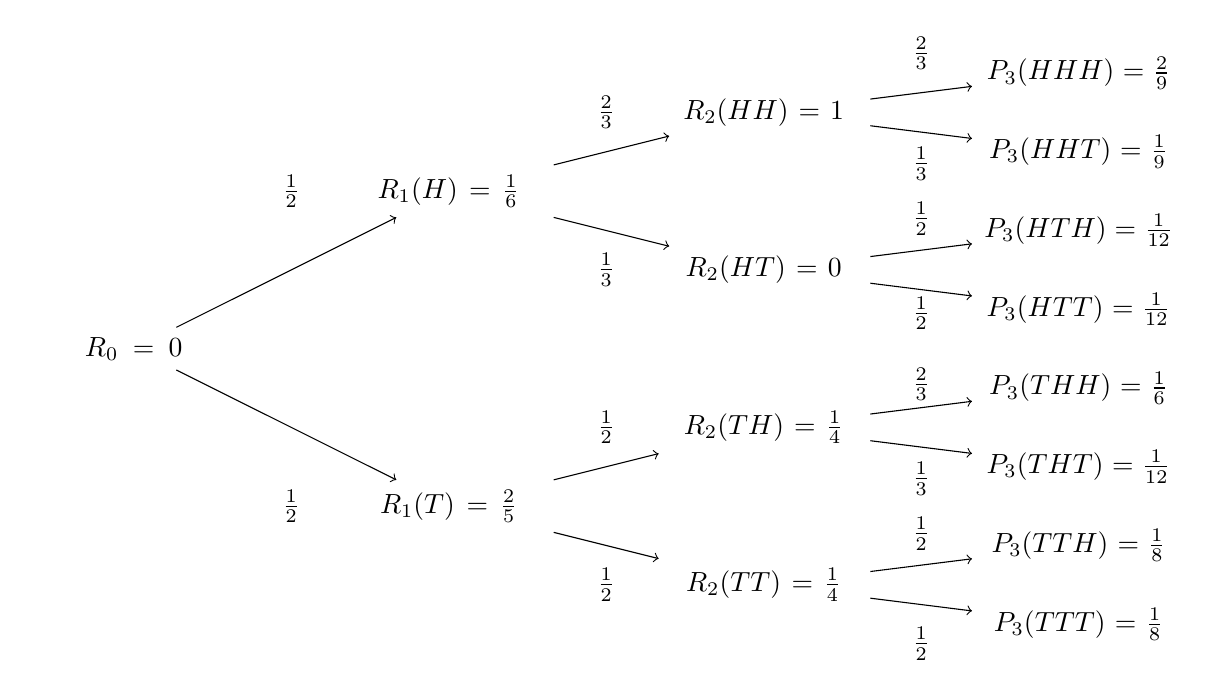
\begin{tikzpicture}[sloped]
  \node (a) at (0,0) [bag] {$R_0 = 0$};
  \node (b) at (4,-2) [bag] {$R_1(T) = \frac{2}{5}$};
  \node (c) at (4,2) [bag] {$R_1(H) = \frac{1}{6}$};
  \node (d) at (8,-3) [bag] {$R_2(TT) = \frac{1}{4}$};
  \node (e) at (8,-1) [bag] {$R_2(TH) = \frac{1}{4}$};
  \node (f) at (8,1) [bag] {$R_2(HT) = 0$};
  \node (g) at (8,3) [bag] {$R_2(HH) = 1$};
  \node (h) at (12,-3.5) [bag] {$P_3(TTT) = \frac{1}{8}$};
  \node (i) at (12,-2.5) [bag] {$P_3(TTH) = \frac{1}{8}$};
  \node (j) at (12,-1.5) [bag] {$P_3(THT) = \frac{1}{12}$};
  \node (k) at (12,-0.5) [bag] {$P_3(THH) = \frac{1}{6}$};
  \node (l) at (12,0.5) [bag] {$P_3(HTT) = \frac{1}{12}$};
  \node (m) at (12,1.5) [bag] {$P_3(HTH) = \frac{1}{12}$};
  \node (n) at (12,2.5) [bag] {$P_3(HHT) = \frac{1}{9}$};
  \node (o) at (12,3.5) [bag] {$P_3(HHH) = \frac{2}{9}$};
  
  \node at (2,-2) {$\frac{1}{2}$};
  \draw [->] (a) to node [below] {} (b);
  \node at (2,2) {$\frac{1}{2}$};  
  \draw [->] (a) to node [above] {} (c);
  \node at (6,-3) {$\frac{1}{2}$};
  \draw [->] (b) to node [below] {} (d);
  \node at (6,-1) {$\frac{1}{2}$};
  \draw [->] (b) to node [above] {} (e);
  \node at (6,1) {$\frac{1}{3}$};
  \draw [->] (c) to node [below] {} (f);
  \node at (6,3) {$\frac{2}{3}$};  
  \draw [->] (c) to node [above] {} (g);
  \node at (10,-3.75) {$\frac{1}{2}$};
  \draw [->] (d) to node [below] {} (h);
  \node at (10,-2.35) {$\frac{1}{2}$};
  \draw [->] (d) to node [above] {} (i);
  \node at (10,-1.65) {$\frac{1}{3}$};
  \draw [->] (e) to node [below] {} (j);
  \node at (10,-0.45) {$\frac{2}{3}$};  
  \draw [->] (e) to node [above] {} (k);
  \node at (10,0.45) {$\frac{1}{2}$};  
  \draw [->] (f) to node [below] {} (l);
  \node at (10,1.65) {$\frac{1}{2}$};
  \draw [->] (f) to node [above] {} (m);
  \node at (10,2.35) {$\frac{1}{3}$};
  \draw [->] (g) to node [above] {} (n);
  \node at (10,3.75) {$\frac{2}{3}$};    
  \draw [->] (g) to node [above] {} (o);  
\end{tikzpicture}
\caption{Interest rate process with conditional transition probabilities annotated above each branch.}
\end{figure}

Note that with
\begin{equation*}
	D_n = \frac{1}{\prod^{n - 1}_{i = 0} (1 + R_i)}
\end{equation*}

we find
\begin{align*}
	D_1 &= \frac{1}{(1 + R_0)} \\
	D_2 &= \frac{1}{(1 + R_0)(1 + R_1)} \\
	D_3 &= \frac{1}{(1 + R_0)(1 + R_1)(1 + R_2)}
\end{align*}

\indent For later use we compute the following quantities depending on the outcome of the coin toss sequence $\omega_1\omega_2 \in \Omega$. Using the tree above we find

\begin{figure}[h!]
\centering
\begin{tabular}{C|CCCCCCC}
	\omega_1\omega_2 & \frac{1}{(1 + R_0)} & \frac{1}{(1 + R_2)} & \frac{1}{(1 + R_2)} & D_1 & D_2 & D_3 & \tilde{\P}(\omega_1\omega_2) \\
	\hline
	HH & 1 & \frac{6}{7} & \frac{1}{2} & 1 & \frac{6}{7} & \frac{3}{7} & \frac{1}{3} \\
	HT & 1 & \frac{6}{7} & 1 & 1 & \frac{6}{7} & \frac{6}{7} & \frac{1}{6} \\
	TH & 1 & \frac{5}{7} & \frac{4}{5} & 1 & \frac{5}{7} & \frac{4}{7} & \frac{1}{4} \\
	TT & 1 & \frac{5}{7} & \frac{4}{5} & 1 & \frac{5}{7} & \frac{4}{7} & \frac{1}{4}
\end{tabular}
\end{figure}

We calculate our time-zero zero-coupon bond prices using
\begin{align*}
	B_{0,n} &= \tilde{\E}_0 \left[ D_n \right] \\
	B_{0,1} &= \tilde{\E}_0 \left[ D_1 \right] \\
	&= \tilde{\E}_0 \left[ \frac{1}{1 + R_0} \right] = \frac{1}{1 + R_0} = 1 \\
	B_{0,2} &= \tilde{\E}_0 \left[ D_2 \right] \\
	&= \sum_{\omega_1} D_2(\omega_1) \tilde{\P}(\omega_1)
	= \frac{1}{2}\cdot \frac{1}{(1 + 0)(1 + \frac{2}{5})} + \frac{1}{2} \cdot \frac{1}{(1 + 0)(1 + \frac{1}{6})} = \frac{11}{14} \\
	B_{0,3} &= \tilde{\E}_0 \left[ D_3 \right] \\
	&= \sum_{\omega_1\omega_2} D_2(\omega_1\omega_2) \tilde{\P}(\omega_1\omega_2) = \frac{1}{3}\cdot\frac{3}{7} + \frac{1}{6}\cdot\frac{6}{7} + \frac{1}{4}\cdot\frac{4}{7} + \frac{1}{4}\cdot\frac{4}{7} = \frac{4}{7}
\end{align*}

and the time-one zero-coupon bond prices are
\begin{align*}
	B_{n,m} &= \tilde{\E}_n \left[ \frac{D_m}{D_n} \right] = \frac{1}{D_n} \tilde{\E}_n \left[D_m\right] \\
	B_{1,1} &= \tilde{\E}_1 \left[ \frac{D_1}{D_1} \right] = 1 \\
	B_{1,2}(H) &= \tilde{\E}_1 \left[ \frac{D_2}{D_1} \right](H) = \frac{1}{D_1(H)} \tilde{\E}_1 \left[ D_2 \right](H) = \frac{1}{D_1(H)} D_2(H) \quad \text{(predictability)} \\
	&= \frac{1}{\frac{1}{(1 + R_0)}} \frac{1}{(1 + R_0)(1 + R_1(H))} = \frac{6}{7} \\
	B_{1,2}(T) &= \frac{5}{7} \quad \text{(similar computation to $B_{1,2}(H)$)}\\
	B_{1,3}(H) &= \frac{1}{D_2(H)} \sum_{\omega_2} D_3(H\omega_2) \tilde{\P}(H\omega_2) = \frac{4}{7} \\
	B_{1,3}(T) &= \frac{1}{D_2(T)} \sum_{\omega_2} D_3(T\omega_2) \tilde{\P}(T\omega_2) = \frac{4}{7} \\
\end{align*}

the time-two zero-coupon bond prices
\begin{align*}
	B_{2,2} &= \tilde{\E}_2 \left[ \frac{D_2}{D_2} \right] = 1 \\
	B_{2,3}(HH) &= \frac{1}{D_2(HH)} \tilde{\E}_2 \left[ D_3 \right](HH) = \frac{D_3(HH)}{D_2(HH)} = \frac{1}{2} \quad \text{(predictability)} \\
	B_{2,3}(HT) &= 1 \\
	B_{2,3}(TH) &= \frac{4}{5} \\
	B_{2,3}(TT) &= \frac{4}{5}
\end{align*}

\indent Consider now a three-period interest rate cap with cap $K = \frac{1}{3}$. The payoff from the caplets (which compose the cap) are
\begin{figure}[h!]
\centering
\begin{tabular}{C|CCCCCC}
	\omega_1\omega_2 & R_0 & (R_0 - \frac{1}{3})^+ & R_1 & (R_1 - \frac{1}{3})^+ & R_2 & (R_2 - \frac{1}{3})^+ \\
	\hline
	HH & 0 & 0 & \frac{1}{6} & 0 & 1 & \frac{2}{3} \\
	HT & 0 & 0 & \frac{1}{6} & 0 & 0 & 0 \\
	TH & 0 & 0 & \frac{2}{5} & \frac{1}{15} & \frac{1}{4} & 0 \\
	TT & 0 & 0 & \frac{2}{5} & \frac{1}{15} & \frac{1}{4} & 0
\end{tabular}
\end{figure}

Then, the time-zero price for the caplet, using the risk-neutral pricing formula, is given by
\begin{align*}
	\tilde{\E}_0 \left[ D_1 \left(R_0 - \frac{1}{3}\right)^+ \right] &= 0 \\
	\tilde{\E}_0 \left[ D_2 \left(R_1 - \frac{1}{3}\right)^+ \right] &= \sum_{\omega_1} D_2(\omega_1) \left(R_1(\omega_1) - \frac{1}{3}\right)^+ \tilde{\P}(\omega_1) \\
	&= \frac{6}{7}\left( \frac{1}{6} - \frac{1}{3}\right)^+\frac{1}{2} + \frac{5}{7}\left( \frac{2}{5} - \frac{1}{3}\right)^+ \frac{1}{2} = \frac{1}{42} \\
	\tilde{\E}_0 \left[ D_3 \left(R_2 - \frac{1}{3}\right)^+ \right] &= \sum_{\omega_1\omega_2} D_3(\omega_1\omega_2) \left( R_2(\omega_1\omega_2) - \frac{1}{3} \right)^+ \tilde{\P}(\omega_1\omega_2) \\
	&= \frac{2}{21}
\end{align*}

Therefore, applying our risk-neutral pricing formula for an $m$-period cap
\begin{equation*}
	\text{Cap}_m = \tilde{\E}_0 \left[ \sum^m_{n = 1} D_n \left(R_{n - 1} - K\right)^+ \right] \quad \text{(the cap is the sum of caplets)}
\end{equation*}

we have
\begin{equation*}
	\text{Cap}_3 = 0 + \frac{1}{42} + \frac{2}{21} = \frac{5}{42}
\end{equation*}

as desired. \\

\underline{Example:} {\em (Exercise 6.4)} Consider the same data as in Example 6.3.9 above. We wish to hedge a short position in the caplet paying $\left( R_2 - \frac{1}{3} \right)^+$ at time $n = 3$. From Example 6.3.9 we have that the time $n = 3$ payoff of the caplets are
\begin{align*}
	V_3(HH) &= \frac{2}{3} \\
	V_3(HT) &= 0 \\
	V_3(TH) &= 0 \\
	V_3(TT) &= 0
\end{align*}

\indent Since $V_3(\omega_1\omega_2)$ depends on only the first two coin tosses, we find that the time-two price of the caplet can be determined by simply discounting the payoffs:
\begin{align*}
	V_2(HH) &= \frac{1}{1 + R_2(HH)}V_3(HH) = \frac{1}{3} \\
	V_2(HT) &= 0 \\
	V_2(TH) &= 0 \\
	V_2(TT) &= 0
\end{align*}

To determine the time-one prices $V_1(H)$ and $V_1(T)$ we compute the risk-neutral expectation
\begin{align*}
	V_1(H) &= \tilde{\E}_1 \left[  \frac{V_2}{1 + R_1} \right](H) \\
	&= \frac{1}{1 + \frac{1}{6}} \left[ \frac{2}{3}\cdot\frac{1}{3} + \frac{1}{3}\cdot 0 \right] = \frac{4}{21} \\
	V_1(T) &= \tilde{\E}_1 \left[  \frac{V_2}{1 + R_1} \right](T) = 0
\end{align*}

\indent We wish to now show that beginning with initial wealth $X_0 = \frac{2}{21}$ and by investing in strictly the money market \& maturity-two bond we may achieve a portfolio value $X_1 = V_1$, regardless of the outcome of $\omega_1$. Note that we have no need for time-three maturity bonds since this would, in principle, the ability to hedge over times two to three. However, the interest rate at time 2 is already known and given by $R_2$! That is, since our model ends at time 3 we have no interest rate risk over the final period. \\

\indent To do so we buy $\Delta_0$ units of the time-two maturity bond. Doing so gives us time-one portfolio value 
\begin{equation*}
	X_1 = \Delta_0 B_{1,2} + (1 + R_0)[X_0 - \Delta_0 B_{0,2}] 
\end{equation*}

Since we require $X_1(\omega) = V_1(\omega)$ for all $\omega \in \Omega$
\begin{align*}
	&\begin{cases}
		\frac{4}{21} = V_1(H) = X_1(H) = \Delta_0 B_{1,2}(H) + (1 + R_0)[X_0 - \Delta_0B_{0,2}] \\
		0 = V_1(T) = X_1(T) = \Delta_0 B_{1,2}(T) + (1 + R_0)[X_0 - \Delta_0B_{0,2}] 
	\end{cases} \\
	\implies &\begin{cases}
		\frac{4}{21} = \Delta_0 \frac{6}{7} + \left[ \frac{2}{21} - \Delta_0 \frac{11}{14}\right] \\
		0 = \Delta_0 \frac{5}{7} + \left[ \frac{2}{21} - \Delta_0 \frac{11}{14} \right] 
	\end{cases} \\
	\implies &\begin{cases}
		\frac{4}{21} = \frac{ \Delta_0 }{14} + \frac{2}{21} \\
		0 = -\frac{ \Delta_0 }{14} + \frac{2}{21}
	\end{cases}
\end{align*}

Solving this system we find 
\begin{equation*}
	\Delta_0 = 14 \cdot \frac{2}{21} = \frac{4}{3}
\end{equation*}

We can verify $\Delta_0 = \frac{4}{3}$ given by
\begin{align*}
	\Delta_0 &= \frac{ V_1(H) - V_1(T) }{ B_{1,2}(H) - B_{1,2}(T) } \\
	&= \frac{ \frac{4}{21} - 0 }{ \frac{6}{7} - \frac{5}{7} } \\
	&= \frac{ \frac{4}{21} }{ \frac{1}{7} } \\
	&= \frac{4}{3}
\end{align*}

Applying the wealth equation again we can find the portfolio process $\Delta_1(\omega)$ such that $X_2 = V_2$ for all $\omega \in \Omega$ with initial wealth $X_1(H)$ and $X_1(T)$ using bonds $B_{2,3}$ and $B_{1,3}$ so that
\begin{equation*}
	V_2 = X_2 = \Delta_1B_{2,3} + (1 + R_1)[X_1 - \Delta_1B_{1,3}]
\end{equation*}

Now, we had that
\begin{equation*}
	V_2(HH) = \frac{1}{3}
\end{equation*}

so then
\begin{align*}
	\frac{1}{3} = V_2(HH) = X_2(HH) &= \Delta_1(H)B_{2,3}(HH) + (1 + R_1(H))[X_1(H) - \Delta_1(H)B_{1,3}(H)] \\
	&= \Delta_1(H)\frac{1}{2} + \frac{7}{6}\left[ \frac{4}{21} - \Delta_1(H)\frac{4}{7}\right] \\
	&= -\frac{1}{6}\Delta_1(H) + \frac{2}{9} \\
	\implies \Delta_1(H) &= -\frac{2}{3}
\end{align*}

\indent Similarly, we may verify that from setting the wealth equation $0 = V_2(HT) = X_2(HT)$ we find that $\Delta_1(H) = -\frac{2}{3}$, as is consistent with our model.

\indent If $\omega_1 = T$ then we should consider $V_2(TH) = X_2(TH)$ and $V_2(TT) = X_2(TT)$. However, since we had found $X_2(TH) = 0 = X_2(TT)$ then we find that
\begin{equation*}
	\Delta_1(T) = 0
\end{equation*}

and so we are still fully hedged if $\omega_1 = T$ without trading additional units of the asset.

\section{Forward Measures}

Let $V_m$ denote the time-$m$ payoff of some interest rate dependent derivative security. From our risk-neutral pricing formula we have that the time-$n$ price of such a derivative is
\begin{equation*}
	V_n = \frac{1}{D_n} \tilde{\E}_n \left[ D_mV_m \right],\quad n = 0,1,...,m
\end{equation*}

\indent However, in order for us to make use of this formula we require the joint condition distribution (conditional with respect to the information up to $n$) of $D_m$ and $V_m$ under $\tilde{\P}$. We make use of the {\bf change-of-measure} technique, generalized from our earlier work, to simplify this risk-neutral formula. Recall we had defined our change-of-measure variable $Z$ such that 
\begin{equation*}
	Z(\omega) = \frac{ \tilde{\P}(\omega) }{ \P(\omega) }
\end{equation*}

so that we may transform a random variable $Y$ from the real-world measure to the risk-neutral, satisfying
\begin{equation*}
	\tilde{\E}[Y] = \E[ZY]
\end{equation*} 

We now introduce the following definition: \\

\begin{definition} Let $1 \leq m \leq N$ be fixed and define
\begin{equation*}
	Z_{m,m} = \frac{ D_m }{ B_{0,m} }
\end{equation*}

and define the \underline{$m$-forward measure} $\tilde{\P}^m$ by
\begin{equation*}
	\tilde{\P}^m(\omega) = Z_{m,m}(\omega)\tilde{\P}(\omega),\quad\forall\,\omega\in\Omega
\end{equation*}
\end{definition}

To quickly convince ourselves that $\tilde{\P}^m$ is indeed a probability measure we note
\begin{align*}
	\tilde{\P}^m(\Omega) &= \sum_{\omega\in\Omega} \tilde{\P}^m(\omega) \\
	&= \sum_{\omega\in\Omega} Z_{m,m}(\omega)\tilde{\P}(\omega) \\
	&= \tilde{\E}_0 \left[ Z_{m,m} \right] \\
	&= \tilde{\E}_0 \left[ \frac{D_m}{B_{0,m}} \right] \\
	&= \frac{1}{B_{0,m}} \tilde{\E}_0 [D_m] \quad \text{(adaptedness of $B_{0,m}$)} \\
	&= 1
\end{align*}


with all other properties just as straightforwardly confirmable. We wish to also generalize the {\em Radon-Nikod{\'y}m} process to the discussion of stochastic interest rates:
\begin{definition} Let $1 \leq m \leq N$ be fixed. With
\begin{equation*}
	Z_{m,m} = \frac{ D_m }{ B_{0,m} }
\end{equation*}

define the \underline{Radon-Nikod{\'y}m process}
\begin{equation*}
	Z_{n,m} = \tilde{\E}_n[Z_{m,m}],\quad n=0,1,...,m
\end{equation*}
\end{definition}

From this definition we find
\begin{align*}
	Z_{n,m} &= \tilde{\E}_n[Z_{m,m}] \\
	&= \tilde{\E}_n \left[ \frac{D_m}{B_{0,m}} \right] \quad \text{(by definition)} \\
	&= \tilde{\E}_n \left[ \frac{D_n}{D_n} \frac{D_m}{B_{0,m}} \right] \\
	&= \frac{D_n}{B_{0,m}} \tilde{\E}_n \left[ \frac{D_m}{D_n} \right] \quad \text{(taking out what is known)} \\
	&= \frac{D_n}{B_{0,m}} B_{n,m} \quad \text{(definition of $B_{n,m}$)}
\end{align*}

\begin{proposition} Let $\tilde{\E}^m_n \left[ \cdot \right]$ denote\footnote{Perhaps a more informative notation would be $\tilde{\E}^{\tilde{\P}^m}_n[\cdot]$, but we abandon this for brevity.} the conditional expectation at time $n$ with respect to the $m$-forward measure $\tilde{\P}^m$. If $V_m$ is a random variable depending on only the first $m$ coin tosses we have
\begin{align*}
	\tilde{\E}_0[Z_{m,m}V_m] &= \sum_{\omega\in\Omega} Z_{m,m}(\omega)V_m(\omega)\tilde{\P}(\omega) \\
	&= \sum_{\omega\in\Omega} V_m(\omega)\tilde{\P}^m(\omega) \\
	&= \tilde{\E}^m_0 [V_m]
\end{align*}

and, in generality we have
\begin{equation*}
	\frac{1}{Z_{n,m}} \tilde{\E}_n[Z_{m,m}V_m] = \tilde{\E}^m_n[V_m], \quad n = 0,1,...,m
\end{equation*}

\indent Since from our earlier lemma,\footnote{Lemma 3.2.6 in Shreve's Stochastic Calculus for Finance I.}~for $0 \leq n \leq m \leq N$, if $Y$ is a random variable depending on only $\omega_1\cdots\omega_m$, then
\begin{equation*}
	\tilde{\E}_n[Y] = \frac{1}{Z_n}\E_n[Z_mY]
\end{equation*}

\indent Hence with $Y = V_m$, $Z_n = Z_{n,m}$, $Z_m = Z_{m,m}$, and $\tilde{\E}_n = \tilde{\E}^m_n$, we find establish our identity, as desired.
\end{proposition} \hfill

\indent We  are now in a position to present a new formulation of the General Bayes' Theorem discussed in previous sections. We have
\begin{theorem}{\bf General Bayes' Theorem II} Let $m$ be fixed such that $1 \leq m \leq N$ and let $\tilde{\P}^m$ be the $m$-forward measure. If $0 \leq n \leq m$ and $V_m$ depends only on the first $m$ coin tosses, then
\begin{equation*}
	\tilde{\E}^m_n[V_m] = \frac{1}{D_nB_{n,m}} \tilde{\E}_n [D_mV_m]
\end{equation*}

\begin{proof} We have
\begin{align*}
	\tilde{\E}^m_n [V_m] &= \frac{1}{Z_{n,m}} \tilde{\E}_n [Z_{m,m}V_m] \quad \text{(from the above proposition)} \\
	&= \frac{ B_{0,m} }{ D_n B_{n,m} } \tilde{\E}_n \left[ \frac{ D_m \overbrace{B_{m,m}}^{=1} }{ B_{0,m} } V_m \right] \quad \text{(by definition of $Z_{n,m}$ and $Z_{m,m}$)} \\
		&= \frac{ 1 }{ B_{n,m} } \tilde{\E}_n \left[ \frac{B_{0,m}}{D_n} \cdot \frac{ D_m }{ B_{0,m} } V_m \right] \quad \text{(``taking in'' what is known)} \\
		&= \frac{ 1 }{ D_nB_{n,m} } \tilde{\E}_n \left[ D_m V_m \right]
\end{align*}

which established our result, as desired. 
\end{proof}
\end{theorem}

\begin{corollary} We may continue with this result to show that $\tilde{\E}^m_n[V_m]$ is the time-$n$ price of any derivative paying $V_m$ at time $m$ {\bf{\em denominated in units of the zero-coupon bond maturing at time m.}} That is, the {\em forward price} of the asset as given by
\begin{equation*}
	Fwd_{n,m} = \frac{ S_n }{B_{n,m}} 
\end{equation*}

\indent We say that the price of an asset denominated this way is a martingale under the $m$-forward measure $\tilde{\P}^m$.

\begin{proof} From the Theorem above
\begin{align*}
\tilde{\E}^m_n [V_m] &= \frac{ 1 }{ D_nB_{n,m} } \tilde{\E}_n \left[ D_m V_m \right] \\
		&= \frac{ 1 }{ B_{n,m} } \tilde{\E}_n \left[ \frac{ V_m }{(1 + R_n)\cdots(1 + R_{m - 1})} \right] \\
		&= \frac{1}{ B_{n,m} } V_n \quad \text{(risk neutral pricing)} 
\end{align*}

\indent In additional the the result, this gives us that the $m$-forward prices of assets are $\tilde{\P}^m$-martingales.
\end{proof}
\end{corollary}

\indent Our application of this result will be that it is sometimes more simple to compute the $m$-forward expectation $\tilde{\E}^m_n[V_m]$ than it is to calculate the risk-neutral expectation $\tilde{\E}_n \left[ \frac{D_m}{D_n} V_m \right]$. In fact, we can see that we may compute the time-$n$ price of our derivative $V_n$ by rearranging our terms to yield
\begin{equation*}
	V_n = B_{n,m} \tilde{\E}^m_n[V_m]
\end{equation*}

\indent This gives us the time-$n$ price of a security paying $V_m$ at time $m$ {\bf denominated in units of the zero-coupon bond maturing at time $m$.} We call this $m$-maturity zero-coupon bond the \underline{num{\'e}raire} for the $m$-forward measure $\tilde{\P}^m$. If we know the distribution of $V$ under $\tilde{\P}^m$ then we don't have to do any discounting under the expectation to arrive to our fair price $V_m$! \\

\underline{Example:} {\em (Exercise 6.5)} Let $0 \leq m \leq N - 1$ be fixed and consider the forward interest rate given by
\begin{equation*}
	F_{n,m} = \frac{ B_{n,m} - B_{n,m + 1} }{ B_{n,m + 1} }, \quad n = 0,1,...,m
\end{equation*}

\indent Show that $F_{n,m}$, for $n = 0,1,...,m$, is a martingale under the $(m + 1)$-forward measure $\tilde{\P}^{m + 1}$. \\

{\em Solution}: Note that both $B_{n,m}$ and $B_{n,m + 1}$ depend only on the first $n$ coin tosses $\omega_1\cdots\omega_n$. Therefore, since $B_{n,m}$ and $B_{n,m + 1}$ are adapted, we find $F_{n,m}$ to be adapted. \\

Now, to test the martingale property under $\tilde{\P}^{m + 1}$:
\begin{align*}
	\tilde{\E}^{m + 1}_n \left[ F_{n + 1,m} \right] &= \frac{1}{D_nB_{n,m + 1}} \tilde{\E}_n \left[ D_{m + 1}F_{n + 1,m} \right] \quad \text{(from Bayes' II)} \\
	&= \frac{ 1 }{B_{n, m  +1}} \tilde{\E}_n \left[ \frac{D_{m + 1}}{D_n} F_{n + 1,m} \right] \quad \text{(predictability of $D_n$)} \\
	&=  \frac{ 1 }{B_{n, m  +1}} \tilde{\E}_n \left[ \frac{D_{m + 1}}{D_n} \left( \frac{ B_{n + 1,m} - B_{n + 1,m + 1} }{ B_{n + 1,m + 1} } \right) \right] \quad \text{(definition)} \\
	&= \frac{ 1 }{B_{n, m  +1}} \left( \tilde{\E}_n \left[ \frac{D_{m + 1}}{D_n} \frac{B_{n + 1,m}}{B_{n + 1,m + 1}} \right] - \tilde{\E}_n \left[ \frac{D_{m + 1}}{D_n} \right] \right) \quad \text{(linearity)} \\
	&= \frac{ 1 }{B_{n, m  +1}} \left( \tilde{\E}_n \left[ \frac{D_{m + 1}}{D_n} \frac{B_{n + 1,m}}{B_{n + 1,m + 1}} \right] - B_{n,m + 1} \right) \quad \text{(definition of $B_{n,m + 1}$)} \\
	&= \frac{ 1 }{B_{n, m  +1}} \left( \tilde{\E}_n \left[ \frac{D_{m + 1}}{D_n} \frac{ \tilde{\E}_{n + 1} \left[ \frac{D_m}{D_{n + 1}} \right] }{ \tilde{\E}_{n + 1} \left[ \frac{D_{m + 1}}{D_{n + 1}} \right] } \right] - B_{n,m + 1} \right) \quad \text{(definition of $B_{n + 1,m}$ and $B_{n + 1,m + 1}$)} \\
	&= \frac{ 1 }{B_{n, m  +1}} \left( \tilde{\E}_n \left[ \frac{D_{m + 1}}{D_n} \frac{ \tilde{\E}_{n + 1} \left[ D_m \right] }{ \tilde{\E}_{n + 1} \left[ D_{m + 1} \right] } \right] - B_{n,m + 1} \right) \quad \text{(predictability of $D_{n + 1}$)}
\end{align*}

However, note that
\begin{align*}
	\tilde{\E}_n \left[ \frac{D_{m + 1}}{D_n} \frac{ \tilde{\E}_{n + 1} \left[ D_m \right] }{ \tilde{\E}_{n + 1} \left[ D_{m + 1} \right] } \right] &= \tilde{\E}_n \left[ \tilde{\E}_{n + 1} \left[ \frac{D_{m + 1}}{D_n} \frac{ \tilde{\E}_{n + 1} \left[ D_m \right] }{ \tilde{\E}_{n + 1} \left[ D_{m + 1} \right] } \right] \right] \quad \text{(tower property)} \\
	&= \tilde{\E}_n \left[ \frac{1}{D_n} \tilde{\E}_{n + 1} \left[ D_{m + 1} \frac{ \tilde{\E}_{n + 1} \left[ D_m \right] }{ \tilde{\E}_{n + 1} \left[ D_{m + 1} \right] } \right] \right] \quad \text{(predictability of $D_n$)} \\
	&= \tilde{\E}_n \left[ \frac{ \tilde{\E}_{n + 1} \left[ D_m \right] }{D_n} \tilde{\E}_{n + 1} \left[ D_{m + 1} \frac{ 1 }{ \tilde{\E}_{n + 1} \left[ D_{m + 1} \right] } \right] \right] \\
	&= \tilde{\E}_n \left[ \frac{ \tilde{\E}_{n + 1} \left[ D_m \right] }{ D_n \tilde{\E}_{n + 1} \left[ D_{m + 1} \right]  } \tilde{\E}_{n + 1} \left[ D_{m + 1} \right] \right] \\
	&= \tilde{\E}_n \left[ \frac{ \tilde{\E}_{n + 1} \left[ D_m \right] }{ D_n } \right] \\
	&= \tilde{\E}_n \left[ \tilde{\E}_{n + 1} \left[ \frac{1}{D_n} D_m \right] \right] \quad \text{(predictability of $D_n$)} \\
	&= \tilde{\E}_n \left[ \frac{D_m}{D_n} \right] \quad \text{(tower property)} \\	
	&= B_{n,m} \quad \text{(definition)}
\end{align*}

Hence
\begin{align*}
	\tilde{\E}^{m + 1}_n \left[ F_{n + 1,m} \right] &= \frac{ 1 }{B_{n, m  +1}} \left( \tilde{\E}_n \left[ \frac{D_{m + 1}}{D_n} \frac{ \tilde{\E}_{n + 1} \left[ D_m \right] }{ \tilde{\E}_{n + 1} \left[ D_{m + 1} \right] } \right] - B_{n,m + 1} \right) \\
	&= \frac{ 1 }{B_{n, m  +1}} \left( B_{n, m} - B_{n,m + 1} \right) \\
	&= F_{n,m}
\end{align*}

Therefore, $\left\{ F_{n,m} \right\}^m_{n = 0}$ is a $\tilde{\P}^{m + 1}$-martingale, as desired.



\end{document}
